\documentclass{standalone}
\usepackage{tikz}
\usetikzlibrary{patterns, positioning}

\begin{document}
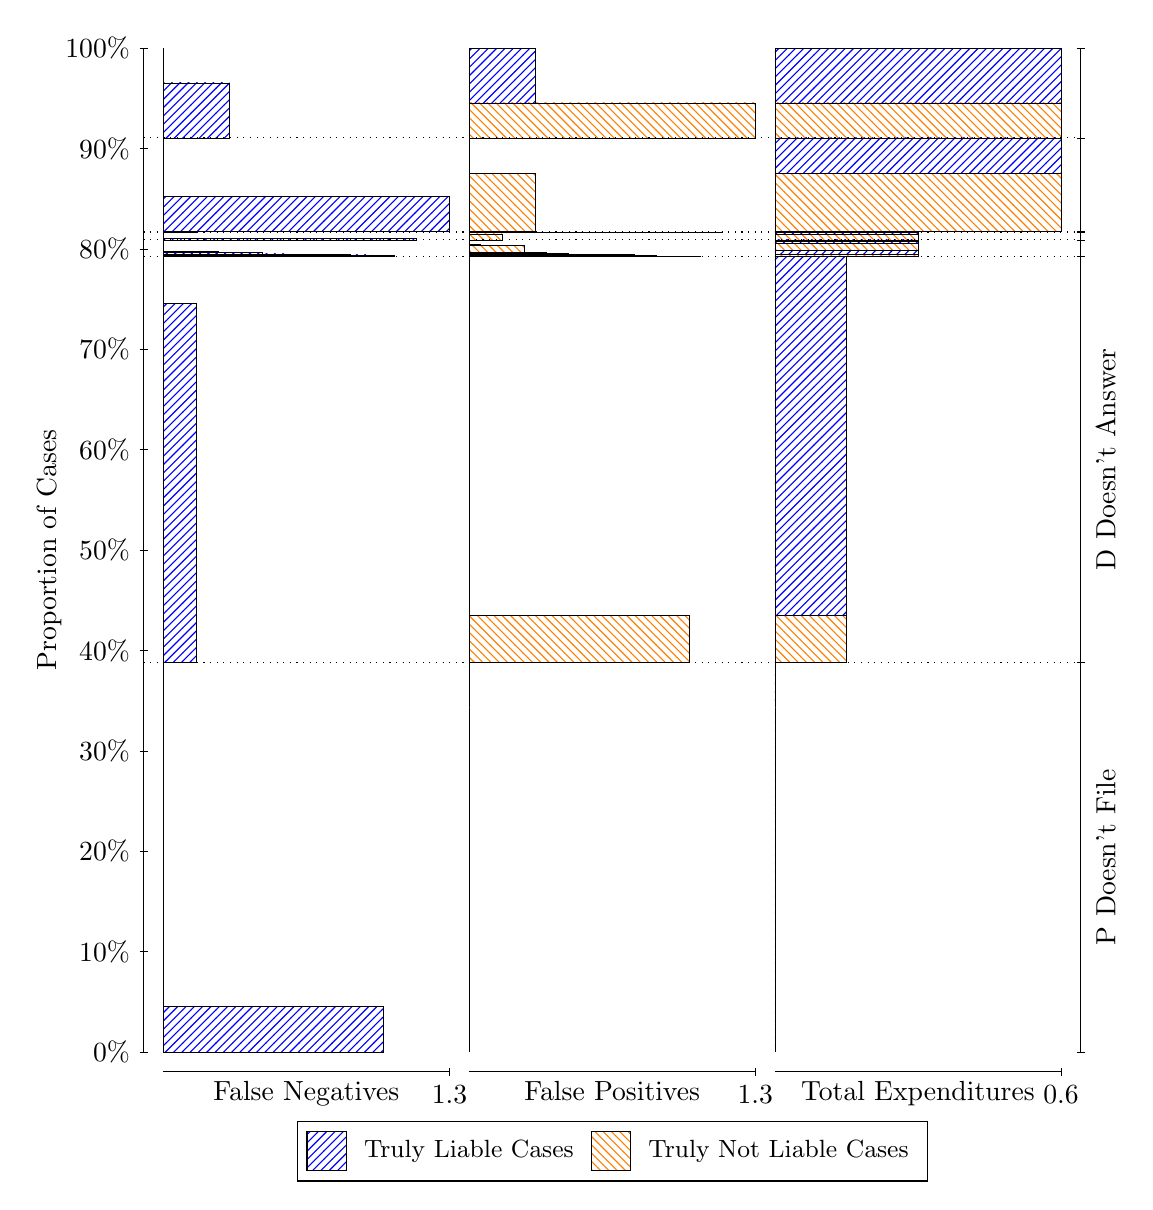
\begin{tikzpicture}
\draw[black, very thin] (1.5,1.75) -- (1.5,14.5);
\node[rotate=90, anchor=center] at (0.3, 8.125) {Proportion of Cases};
\draw[black, very thin] (1.45,1.75) -- (1.55,1.75);
\node[anchor=east] at (1.45, 1.75) {0\%};
\draw[black, very thin] (1.45,3.025) -- (1.55,3.025);
\node[anchor=east] at (1.45, 3.025) {10\%};
\draw[black, very thin] (1.45,4.3) -- (1.55,4.3);
\node[anchor=east] at (1.45, 4.3) {20\%};
\draw[black, very thin] (1.45,5.575) -- (1.55,5.575);
\node[anchor=east] at (1.45, 5.575) {30\%};
\draw[black, very thin] (1.45,6.85) -- (1.55,6.85);
\node[anchor=east] at (1.45, 6.85) {40\%};
\draw[black, very thin] (1.45,8.125) -- (1.55,8.125);
\node[anchor=east] at (1.45, 8.125) {50\%};
\draw[black, very thin] (1.45,9.4) -- (1.55,9.4);
\node[anchor=east] at (1.45, 9.4) {60\%};
\draw[black, very thin] (1.45,10.675) -- (1.55,10.675);
\node[anchor=east] at (1.45, 10.675) {70\%};
\draw[black, very thin] (1.45,11.95) -- (1.55,11.95);
\node[anchor=east] at (1.45, 11.95) {80\%};
\draw[black, very thin] (1.45,13.225) -- (1.55,13.225);
\node[anchor=east] at (1.45, 13.225) {90\%};
\draw[black, very thin] (1.45,14.5) -- (1.55,14.5);
\node[anchor=east] at (1.45, 14.5) {100\%};

\draw[black, very thin] (13.4,1.75) -- (13.4,14.5);
\draw[black, very thin] (13.35,1.75) -- (13.45,1.75);
\node[anchor=west] at (13.35, 1.75) {};
\draw[black, very thin] (13.35,6.6987) -- (13.45,6.6987);
\node[anchor=west] at (13.35, 6.6987) {};
\draw[black, very thin] (13.35,11.851) -- (13.45,11.851);
\node[anchor=west] at (13.35, 11.851) {};
\draw[black, very thin] (13.35,12.063) -- (13.45,12.063);
\node[anchor=west] at (13.35, 12.063) {};
\draw[black, very thin] (13.35,12.156) -- (13.45,12.156);
\node[anchor=west] at (13.35, 12.156) {};
\draw[black, very thin] (13.35,12.169) -- (13.45,12.169);
\node[anchor=west] at (13.35, 12.169) {};
\draw[black, very thin] (13.35,13.359) -- (13.45,13.359);
\node[anchor=west] at (13.35, 13.359) {};
\draw[black, very thin] (13.35,14.5) -- (13.45,14.5);
\node[anchor=west] at (13.35, 14.5) {};

\draw[black, very thin, pattern color=blue, pattern=north east lines] (1.75,1.75) rectangle (4.5449,2.3247);
\draw[black, very thin, pattern color=orange, pattern=north west lines] (1.75,2.3247) rectangle (1.75,6.6987);
\draw[black, very thin, pattern color=blue, pattern=north east lines] (1.75,6.6987) rectangle (2.1692,11.255);
\draw[black, very thin, pattern color=orange, pattern=north west lines] (1.75,11.255) rectangle (1.75,11.851);
\draw[black, very thin, pattern color=blue, pattern=north east lines] (1.75,11.851) rectangle (4.6846,11.869);
\draw[black, very thin, pattern color=blue, pattern=north east lines] (1.75,11.869) rectangle (4.4051,11.873);
\draw[black, very thin, pattern color=blue, pattern=north east lines] (1.75,11.873) rectangle (4.1256,11.875);
\draw[black, very thin, pattern color=blue, pattern=north east lines] (1.75,11.875) rectangle (3.8462,11.876);
\draw[black, very thin, pattern color=blue, pattern=north east lines] (1.75,11.876) rectangle (3.5667,11.883);
\draw[black, very thin, pattern color=blue, pattern=north east lines] (1.75,11.883) rectangle (3.2872,11.887);
\draw[black, very thin, pattern color=blue, pattern=north east lines] (1.75,11.887) rectangle (3.0077,11.904);
\draw[black, very thin, pattern color=blue, pattern=north east lines] (1.75,11.904) rectangle (2.7282,11.907);
\draw[black, very thin, pattern color=blue, pattern=north east lines] (1.75,11.907) rectangle (2.4487,11.922);
\draw[black, very thin, pattern color=orange, pattern=north west lines] (1.75,11.922) rectangle (1.75,12.063);
\draw[black, very thin, pattern color=blue, pattern=north east lines] (1.75,12.063) rectangle (4.9641,12.079);
\draw[black, very thin, pattern color=orange, pattern=north west lines] (1.75,12.079) rectangle (1.75,12.156);
\draw[black, very thin, pattern color=blue, pattern=north east lines] (1.75,12.156) rectangle (2.1692,12.167);
\draw[black, very thin, pattern color=orange, pattern=north west lines] (1.75,12.167) rectangle (1.75,12.169);
\draw[black, very thin, pattern color=blue, pattern=north east lines] (1.75,12.169) rectangle (5.3833,12.618);
\draw[black, very thin, pattern color=orange, pattern=north west lines] (1.75,12.618) rectangle (1.75,13.359);
\draw[black, very thin, pattern color=blue, pattern=north east lines] (1.75,13.359) rectangle (2.5885,14.058);
\draw[black, very thin, pattern color=orange, pattern=north west lines] (1.75,14.058) rectangle (1.75,14.5);
\draw[black, very thin, pattern color=orange, pattern=north west lines] (5.6333,1.75) rectangle (5.6333,6.124);
\draw[black, very thin, pattern color=blue, pattern=north east lines] (5.6333,6.124) rectangle (5.6333,6.6987);
\draw[black, very thin, pattern color=orange, pattern=north west lines] (5.6333,6.6987) rectangle (8.4282,7.2954);
\draw[black, very thin, pattern color=blue, pattern=north east lines] (5.6333,7.2954) rectangle (5.6333,11.851);
\draw[black, very thin, pattern color=orange, pattern=north west lines] (5.6333,11.851) rectangle (8.5679,11.854);
\draw[black, very thin, pattern color=orange, pattern=north west lines] (5.6333,11.854) rectangle (8.2885,11.855);
\draw[black, very thin, pattern color=orange, pattern=north west lines] (5.6333,11.855) rectangle (8.009,11.871);
\draw[black, very thin, pattern color=orange, pattern=north west lines] (5.6333,11.871) rectangle (7.7295,11.875);
\draw[black, very thin, pattern color=orange, pattern=north west lines] (5.6333,11.875) rectangle (7.45,11.882);
\draw[black, very thin, pattern color=orange, pattern=north west lines] (5.6333,11.882) rectangle (7.1705,11.883);
\draw[black, very thin, pattern color=orange, pattern=north west lines] (5.6333,11.883) rectangle (7.1705,11.884);
\draw[black, very thin, pattern color=orange, pattern=north west lines] (5.6333,11.884) rectangle (6.891,11.889);
\draw[black, very thin, pattern color=orange, pattern=north west lines] (5.6333,11.889) rectangle (6.6115,11.9);
\draw[black, very thin, pattern color=orange, pattern=north west lines] (5.6333,11.9) rectangle (6.3321,11.992);
\draw[black, very thin, pattern color=blue, pattern=north east lines] (5.6333,11.992) rectangle (5.7731,12.007);
\draw[black, very thin, pattern color=blue, pattern=north east lines] (5.6333,12.007) rectangle (5.6333,12.063);
\draw[black, very thin, pattern color=orange, pattern=north west lines] (5.6333,12.063) rectangle (6.0526,12.14);
\draw[black, very thin, pattern color=blue, pattern=north east lines] (5.6333,12.14) rectangle (5.6333,12.156);
\draw[black, very thin, pattern color=orange, pattern=north west lines] (5.6333,12.156) rectangle (8.8474,12.158);
\draw[black, very thin, pattern color=blue, pattern=north east lines] (5.6333,12.158) rectangle (6.0526,12.169);
\draw[black, very thin, pattern color=orange, pattern=north west lines] (5.6333,12.169) rectangle (6.4718,12.91);
\draw[black, very thin, pattern color=blue, pattern=north east lines] (5.6333,12.91) rectangle (5.6333,13.359);
\draw[black, very thin, pattern color=orange, pattern=north west lines] (5.6333,13.359) rectangle (9.2667,13.802);
\draw[black, very thin, pattern color=blue, pattern=north east lines] (5.6333,13.802) rectangle (6.4718,14.5);
\draw[black, very thin, pattern color=orange, pattern=north west lines] (9.5167,1.75) rectangle (9.5167,6.124);
\draw[black, very thin, pattern color=blue, pattern=north east lines] (9.5167,6.124) rectangle (9.5167,6.6987);
\draw[black, very thin, pattern color=orange, pattern=north west lines] (9.5167,6.6987) rectangle (10.425,7.2954);
\draw[black, very thin, pattern color=blue, pattern=north east lines] (9.5167,7.2954) rectangle (10.425,11.851);
\draw[black, very thin, pattern color=orange, pattern=north west lines] (9.5167,11.851) rectangle (11.333,11.883);
\draw[black, very thin, pattern color=blue, pattern=north east lines] (9.5167,11.883) rectangle (11.333,11.929);
\draw[black, very thin, pattern color=orange, pattern=north west lines] (9.5167,11.929) rectangle (11.333,12.022);
\draw[black, very thin, pattern color=blue, pattern=north east lines] (9.5167,12.022) rectangle (11.333,12.04);
\draw[black, very thin, pattern color=orange, pattern=north west lines] (9.5167,12.04) rectangle (11.333,12.057);
\draw[black, very thin, pattern color=blue, pattern=north east lines] (9.5167,12.057) rectangle (11.333,12.063);
\draw[black, very thin, pattern color=orange, pattern=north west lines] (9.5167,12.063) rectangle (11.333,12.14);
\draw[black, very thin, pattern color=blue, pattern=north east lines] (9.5167,12.14) rectangle (11.333,12.156);
\draw[black, very thin, pattern color=orange, pattern=north west lines] (9.5167,12.156) rectangle (11.333,12.158);
\draw[black, very thin, pattern color=blue, pattern=north east lines] (9.5167,12.158) rectangle (11.333,12.169);
\draw[black, very thin, pattern color=orange, pattern=north west lines] (9.5167,12.169) rectangle (13.15,12.91);
\draw[black, very thin, pattern color=blue, pattern=north east lines] (9.5167,12.91) rectangle (13.15,13.359);
\draw[black, very thin, pattern color=orange, pattern=north west lines] (9.5167,13.359) rectangle (13.15,13.802);
\draw[black, very thin, pattern color=blue, pattern=north east lines] (9.5167,13.802) rectangle (13.15,14.5);
\draw[black, dotted] (1.5,6.6987) -- (13.4,6.6987);
\draw[black, dotted] (1.5,11.851) -- (13.4,11.851);
\draw[black, dotted] (1.5,12.063) -- (13.4,12.063);
\draw[black, dotted] (1.5,12.156) -- (13.4,12.156);
\draw[black, dotted] (1.5,12.169) -- (13.4,12.169);
\draw[black, dotted] (1.5,13.359) -- (13.4,13.359);
\draw[black, very thin] (1.75,1.5) -- (5.3833,1.5);
\node[anchor=north] at (3.5667, 1.5) {False Negatives};
\draw[black, very thin] (5.3833,1.45) -- (5.3833,1.55);
\node[anchor=north] at (5.3833, 1.45) {1.3};

\draw[black, very thin] (5.6333,1.5) -- (9.2667,1.5);
\node[anchor=north] at (7.45, 1.5) {False Positives};
\draw[black, very thin] (9.2667,1.45) -- (9.2667,1.55);
\node[anchor=north] at (9.2667, 1.45) {1.3};

\draw[black, very thin] (9.5167,1.5) -- (13.15,1.5);
\node[anchor=north] at (11.333, 1.5) {Total Expenditures};
\draw[black, very thin] (13.15,1.45) -- (13.15,1.55);
\node[anchor=north] at (13.15, 1.45) {0.6};

\node[black, centered, rotate=90] at (13.72, 4.2244) {P Doesn't File};
\node[black, centered, rotate=90] at (13.72, 9.275) {D Doesn't Answer};






\draw (7.449999999999999,1.5) node[draw=none] (baseCoordinate) {};
\begin{scope}[align=center]
        \matrix[scale=0.5, draw=black, below=0.5cm of baseCoordinate, nodes={draw}, column sep=0.1cm]{
            \node[rectangle, draw, minimum width=0.5cm, minimum height=0.5cm, pattern=north east lines, pattern color=blue] {}; &
            \node[draw=none, font=\small] (B) {Truly Liable Cases}; &
            \node[rectangle, draw, minimum width=0.5cm, minimum height=0.5cm, pattern=north west lines, pattern color=orange] {}; &
            \node[draw=none, font=\small] (B) {Truly Not Liable Cases}; \\
            };
\end{scope}

\end{tikzpicture}
\end{document}